\documentclass[prb,twocolumn]{revtex4-2}
\usepackage{graphicx}
\usepackage{amsmath}
\usepackage{amssymb}
\usepackage{epstopdf}

\begin{document}
\title{Assignment 4}

\author{James Lawton}
\affiliation {
Physics Department, Virginia Tech, Blacksburg, Virginia 24061, USA\\
}


\begin{abstract}
Absract: A few sentences summarizing the topics of each problem.  The document should be in APS PRB format.  
\end{abstract}

\maketitle

\section{Problem 1}

\noindent

Here I look to solve the following equation using the Numerov Algorithm:
$$ u"(x)=-4\pi^2u(x)$$
I created a python simulation that ran the algorithm along with an equivatent sine curve to compare to. The Numerov simulation is plotted in black and the sine curve in blue.

\begin{figure}[h!]
\centerline{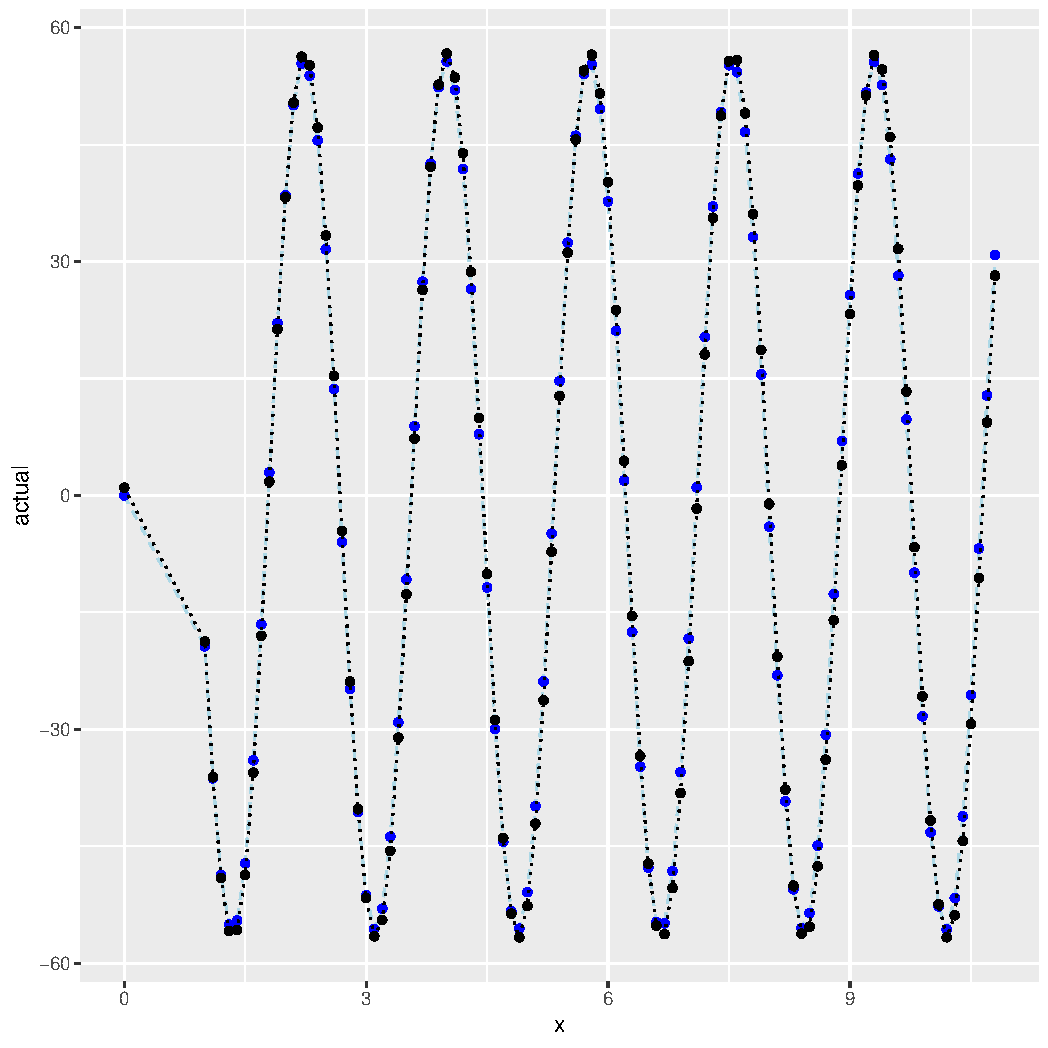
\includegraphics [width=3 in] {q1}} \caption{Numerov vs. x} \label{q1}
\end{figure}

\section{Problem 2}
\section{Problem 3}
\subsection{a}
\subsection{b}
\subsection{c}

\begin{thebibliography}{99}

\bibitem{thecoursetext} T. Pang, \emph{Introduction to Computational Physics}, Cambridge University Press (2006).

\end{thebibliography}

\end{document}
